\documentclass{oblivoir}
\usepackage{graphicx}
\usepackage{mathtools}
\usepackage[left=3.5cm,right=3.5cm,top=3cm,bottom=3cm,a4paper]{geometry}
\usepackage[dvipsnames,svgnames,x11names]{xcolor}
\title{프로그래밍\,I 복습과제 \#1}
\author{1208 이승민}

\begin{document}
\maketitle
\tableofcontents

\section{문제 제기}
\hspace{10pt} 우리는 지난 시간에 개선된 숫자 뒤집기 방법을 배웠다. 이는 상용로그와 제곱을 이용한 방법의 개선된 버전으로, 재귀함수의 호출 횟수를 줄여 시간을 줄이는 아이디어가 사용되었다. 그러나 이 방법에는 오류가 존재했다. 지금부터 오류를 찾고 코드를 올바르게 수정하겠다.
\\

\begin{figure}[ht]
\centering
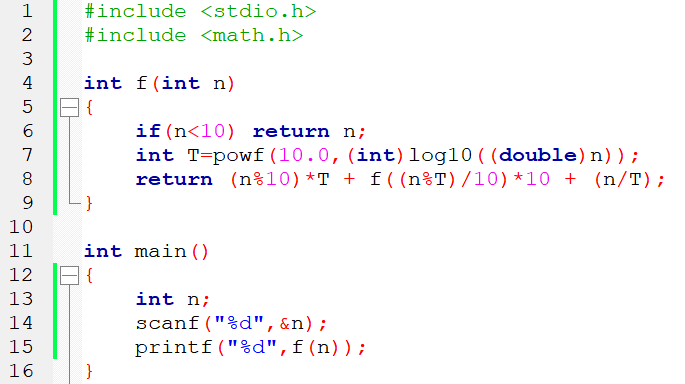
\includegraphics[scale=0.7]{before.png}
\caption{수정 전 코드}
\end{figure}

\section{해결}

\subsection{오류가 발생한 원인을 예를 들어 설명하라.}
\hspace{10pt} 프로그램을 실행한 후 ``10201''을 입력했다. 정상적인 코드라면 입력값과 같은 ``{\color{Green}10201}''을 출력해야 하나, 출력값은 ``{\color{Red}10021}'' 이었다. 먼저 코드의 진행 과정을 살펴보자.	

\begin{enumerate}
\item 10201이 입력되어 15번째 줄에서 $f(10201)$의 값을 구함.
\item 6번째 줄에서 10201$<$10이 아니므로 7번째 줄로 넘어감.
\item 7번째 줄에서 $T_1=10^{\left[ \,log_{10}10201 \right]} = 10^4$이 저장됨. (편의상 $T_1$으로 표기)
\item 8번째 줄에서 $(10201\,\bmod\,10)\times T_1 = 10000$이고, $f(\left[ 10201\,\bmod\,T_1)/10 \right]) = f(20)$의 값을 구함.
\item 6번째 줄에서 20$<$10이 아니므로 7번째 줄로 넘어감.
\item 7번째 줄에서 $T_2=10^{\left[ \,log_{10}20 \right]} = 10$이 저장됨.
\item 8번째 줄에서 $(20\,\bmod\,10)\times T_2 = 0$이고, $f(\left[ 20\,\bmod\,T_2)/10 \right]) = f(0)$의 값을 구함.
\item 6번째 줄에서 0$<$10이므로 0을 $return$.
\item 7로 돌아가 $0 + 0\times 10 + \left[ 20\slash T_2 \right] = 2$를 계산해 $return$.
\item 4로 돌아가 $10000 + 2\times 10 + \left[ 10201\slash T_1 \right] = 10021$을 계산해 $return$.
\end{enumerate}

코드를 살펴보면 4번째 줄에서 문제점을 발견할 수 있다. 코드를 구성한 아이디어대로라면 4번째 줄에서 $f(20)$이 아닌 $f(020)$을 호출해야 한다. 그러나 코드에서는 계산 과정에서 앞의 0을 무시하고 $f(20)$을 호출했고, 이로 인해 ``{\color{Red}20}''을 뒤집은 숫자인 ``{\color{Red}02}''가 되돌아왔다. (원래대로라면  ``{\color{Green}020}''을 뒤집은 숫자인 ``{\color{Green}020}''이 되돌아와야 한다.)
\\

\begin{center}
\begin{tabular}{c|c|c}\hline
과정 & 기존 코드 & 정답 \\\hline\hline
0 & 10201 & 10201 \\
1 & {\color{Red}10201} & {\color{Green}10201} \\
2 & 1{\color{Red}020}1 & 1{\color{Green}020}1 \\
3 & 10{\color{Red}20}1 & 1{\color{Green}020}1 \\
4 & 10{\color{Red}02}1 & 10{\color{Green}2}01 \\
5 & 10021 & 10201 \\
\end{tabular}
\end{center} 
\vspace{10pt}

코드의 진행과정을 대략적으로 나타내었다. (기존 코드의 2,3 과정은 동시에 진행된다.)

\subsection{프로그램을 오류가 없도록 수정하는 과정을 설명하라.}
\hspace{10pt} 오류가 발생한 원인은 4번째 줄에서 앞의 0을 무시하고 $f(20)$을 호출했기 때문이었다. 이를 해결하기 위해서 $f(20)$을 호출하되, 호출할 때 자릿수 정보를 같이 넘겨주면 된다는 아이디어를 생각할 수 있다.\footnote{``020''의 경우에는 $n$값은 20을, 자릿수값은 3을 넘겨주게 된다.} 넘겨주는 자릿수는 입력된 수의 자릿수에서 2를 빼서 넘겨주면 된다. (맨 앞자리의 수와 맨 뒷자리의 수를 제외한 수에 대해 재귀함수를 호출하는 것이기 때문이다.)


다만 계산 과정에서 T가 사용되므로, 자릿수가 아닌 T를 활용해서 재귀함수를 설정하는 것이 간편하다.\footnote{$T = 10^{J-1}$ ($J$:자릿수) 이므로 가능하다.} 
이 경우 T/100을 넘겨주면 된다.

그러나 이러한 방법을 선택할 경우 자릿수가 2 단위로 줄어들게 된다. 따라서 이전의 코드처럼 $n$이 10 이하일 때 $n$을 그대로 돌려주는 것이 아닌, 자릿수가 1일 때와 2일 때 돌려주는 방법을 따로 생각해야 한다. \footnote{자릿수가 1일 때와 2일 때는 각각 $T=1$일 때와 $T=10$일 때를 의미한다.} 

자릿수가 1일 때는 $n$을 그대로 $return$하고, 자릿수가 2일 때는 $n$을 뒤집은 수를 $return$하면 된다.   (두 자리 수 $n$을 뒤집은 수는 $(n\,\bmod\,10)\times 10 + \left[ n/10 \right]$이다.)

$1\leq n\leq 50000$이므로 0이 입력되는 경우에 대해서는 고려할 필요 없다.

\subsection{완성된 프로그램 코드를 제시하라.}
\hspace{10pt} 완성된 프로그램 코드는 다음과 같다.
\\

\begin{figure}[ht]
\centering
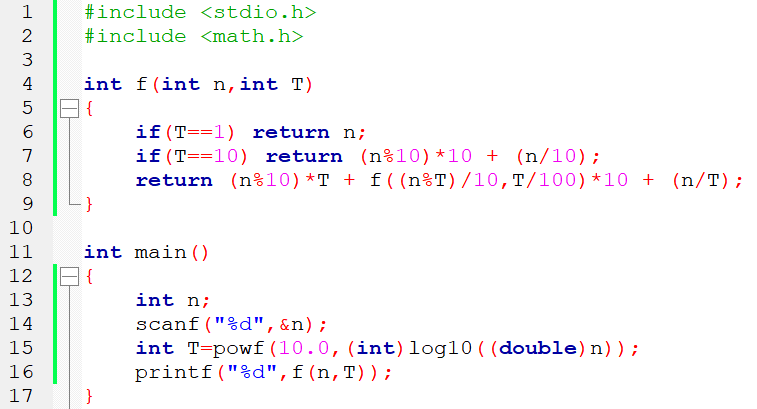
\includegraphics[scale=0.7]{after.png}
\caption{완성된 코드}
\end{figure}



\end{document}